%% Cojinete hidrodinámico con cambio de temperatura (C)
\item Se utiliza un cojinete hidrodinámico como el de la figura \ref{fig:cojinete}
para soportar un eje en rotación a una velocidad angular $\omega$. El aceite empleado tiene una viscosidad que varía con linealmente con la temperatura
$\mu(T) = \mu_0 + c_\mu (T - T_0)$. El área mojada del eje es un cilindro
de radio $R$ y longitud $L$. Como el cojinete funciona
\textit{a régimen}, puede suponer que la película de aceite tiene un espesor
constante $e$.
\\
Por otra parte, la potencia disipada por efecto viscoso es igual al calor transferido
por convección desde el aceite a la caja del cojinete. Dicho calor puede calcularse
por la ley de Newton.
\begin{equation*}
Q = h_c\,A(T - T_{caja})
\end{equation*}
\\
Donde $h_c$ es el coeficiente pelicular de convección, que puede extraerse de tablas.
Considerando que la temperatura $T_{caja}$ es igual a $T_0$, determine la
temperatura de trabajo del aceite como función de los parámetros del problema:
\begin{equation*}
T = T(\omega, R, L, e, \mu_0, c_\mu, T_0, h_c)
\end{equation*}


\begin{figure}[h!!!!]
  \centering
  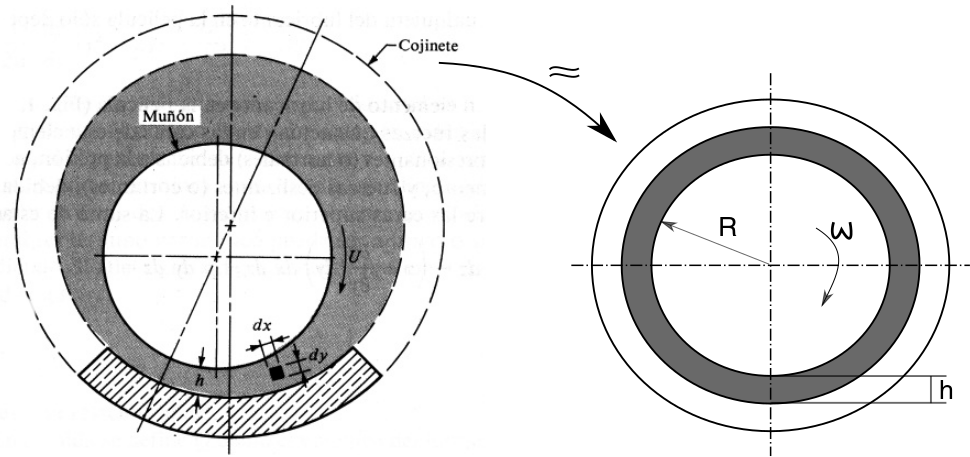
\includegraphics[width=0.7\textwidth]{cojinete.png}
  \caption{Cojinete hidrodinámico trabajando a régimen (esquema adaptado:
  Dudley 1962)}
  \label{fig:cojinete}
\end{figure}
